\documentclass[11pt,a4paper]{article}
\usepackage[margin=2.2cm]{geometry}
\usepackage[T1]{fontenc}
\usepackage[expansion=false]{microtype}
\usepackage{booktabs}
\usepackage{tabularx}
\usepackage{array}
\usepackage{enumitem}
\usepackage{xcolor}
\usepackage{listings}
\usepackage{tikz}
\usetikzlibrary{arrows.meta,positioning}
\usepackage{hyperref}
\usepackage{parskip}
\usepackage{amsmath}

\definecolor{accent}{RGB}{0,51,102}
\definecolor{codebg}{RGB}{245,246,248}
\definecolor{boxbg}{RGB}{235,242,250}
\hypersetup{colorlinks=true,linkcolor=accent,urlcolor=accent}

\lstset{
  basicstyle=\ttfamily\small,
  backgroundcolor=\color{codebg},
  frame=single,
  rulecolor=\color{codebg},
  columns=fullflexible,
  keepspaces=true,
  breaklines=true,
  showstringspaces=false,
  xleftmargin=4pt,
  xrightmargin=4pt,
  aboveskip=6pt,
  belowskip=6pt
}

\newcommand{\file}[1]{\texttt{#1}}
\newcommand{\cmd}[1]{\texttt{#1}}

\setlist{itemsep=2pt,topsep=4pt}
\setlength{\emergencystretch}{3em}

\title{\color{accent}\textbf{ProEm: A Beginner's Guide to the Toolchain}\\[4pt]
\large YAML, simulation, Icarus Verilog, cocotb, the ASIC flow, processes and Tiny Tapeout}
\author{Paul Vincent Bezzina}
\date{28 September 2026}

\begin{document}
\maketitle

\begin{abstract}
This guide explains, from the beginning, every tool and file that takes ProEm from SystemVerilog to a chip. It assumes you know Verilog from Quartus and ModelSim, but not the open-source ASIC world. Each section explains one idea in general terms, then shows exactly where it appears in the ProEm repository. The last sections are a checklist of what to do next and a glossary.
\end{abstract}

\tableofcontents
\newpage

%=====================================================================
\section{The big picture}

An FPGA is a chip that already exists; Quartus configures it. An ASIC is a chip that does not exist yet: the tools must decide where every transistor goes and draw the photographic masks a factory uses to make it. The output of that process is a \textbf{GDS file}, a drawing of every layer of the chip.

The journey for ProEm has two branches that meet at the end: one checks the design works (simulation), the other turns it into a layout (the ASIC flow).

\begin{center}
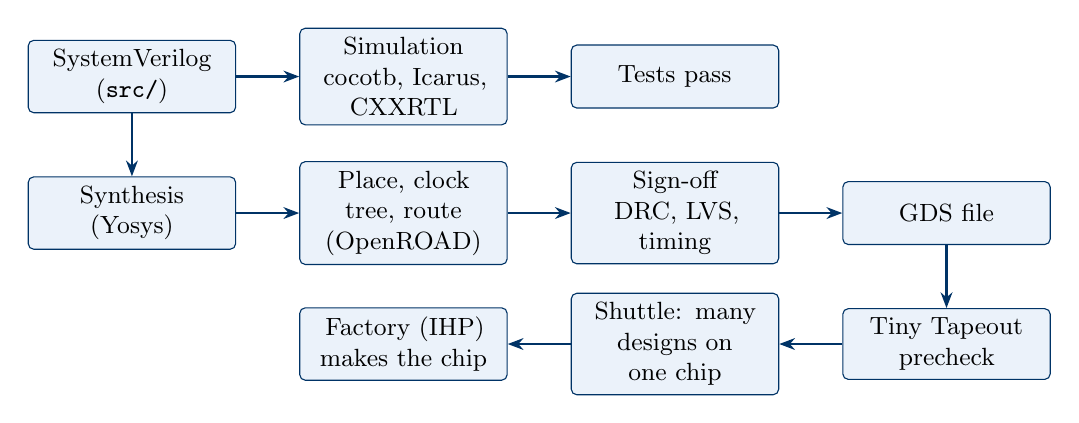
\begin{tikzpicture}[
  box/.style={draw=accent,fill=boxbg,rounded corners=2pt,minimum height=8mm,text width=24mm,align=center,font=\small},
  arr/.style={-{Stealth[length=2mm]},thick,accent}]
\node[box] (rtl) {SystemVerilog\\(\file{src/})};
\node[box,right=8mm of rtl] (sim) {Simulation\\cocotb, Icarus, CXXRTL};
\node[box,right=8mm of sim] (ok) {Tests pass};
\node[box,below=8mm of rtl] (syn) {Synthesis\\(Yosys)};
\node[box,right=8mm of syn] (pnr) {Place, clock tree, route (OpenROAD)};
\node[box,right=8mm of pnr] (sign) {Sign-off\\DRC, LVS, timing};
\node[box,right=8mm of sign] (gds) {GDS file};
\node[box,below=8mm of gds] (pre) {Tiny Tapeout precheck};
\node[box,left=8mm of pre] (shut) {Shuttle: many designs on one chip};
\node[box,left=8mm of shut] (fab) {Factory (IHP) makes the chip};
\draw[arr] (rtl) -- (sim); \draw[arr] (sim) -- (ok);
\draw[arr] (rtl) -- (syn); \draw[arr] (syn) -- (pnr); \draw[arr] (pnr) -- (sign); \draw[arr] (sign) -- (gds);
\draw[arr] (gds) -- (pre); \draw[arr] (pre) -- (shut); \draw[arr] (shut) -- (fab);
\end{tikzpicture}
\end{center}

For you, almost all of this runs automatically: when you push to GitHub, \textbf{GitHub Actions} (computers GitHub lends you) run the tests and the whole ASIC flow, and show a green tick or a red cross. Your job is to write the SystemVerilog, keep the tests passing, and make sure the \cmd{gds} run is green. Jane Street's email says exactly this: start from the CMOS5L template, let the Tiny Tapeout Actions build the GDS and run the precheck, and submit a design with a passing build.

%=====================================================================
\section{The files in your repository}

\begin{center}
\begin{tabularx}{\linewidth}{@{}lX@{}}
\toprule
File or folder & What it is for \\
\midrule
\file{src/} & Your SystemVerilog. \file{top/tt\_um\_vertrex\_star\_proem.sv} is the Tiny Tapeout wrapper; everything else sits under it. \\
\file{src/config.json} & Settings for the ASIC flow (LibreLane): clock period, placement density, timing margins. Section~\ref{sec:json}. \\
\file{info.yaml} & The Tiny Tapeout project description: name, top module, tile size, source files, pin names. Section~\ref{sec:yaml}. \\
\file{test/} & The cocotb test: \file{test.py} (Python), \file{tb.v} (a Verilog wrapper), \file{Makefile}, \file{requirements.txt}. Section~\ref{sec:cocotb}. \\
\file{sim/}, \file{scripts/run.sh} & The larger C++ test suite (CXXRTL): 13 pin-level tests plus random programs. Section~\ref{sec:cxxrtl}. \\
\file{.github/workflows/} & The recipes GitHub Actions follow on every push: \file{gds.yaml}, \file{test.yaml}, \file{sim.yaml}, \file{docs.yaml}. Section~\ref{sec:actions}. \\
\file{docs/} & The ISA and design documents, the datasheet page \file{info.md}, diagrams. \\
\file{gds/} & A copy of the finished layout (GDS, LEF), images, and a results summary. \\
\file{host/} & The Python host library (\file{proem\_host.py}) that builds instruction bytes and decodes replies, and a README on how to drive the chip. \\
\file{formal/} & Formal proofs: harnesses and \file{.sby} files for SymbiYosys (see the separate formal verification guide). \\
\bottomrule
\end{tabularx}
\end{center}

%=====================================================================
\section{YAML}\label{sec:yaml}

\subsection{What YAML is}

YAML is a plain-text format for writing down structured settings that both people and programs can read. It has only three building blocks:

\begin{itemize}
\item \textbf{A value}: text or a number, such as \texttt{50000000} or \texttt{"6x4"}.
\item \textbf{A map} (also called a dictionary): names paired with values, written \texttt{name: value}.
\item \textbf{A list}: items written one per line, each starting with a dash \texttt{-}.
\end{itemize}

Nesting is shown by \textbf{indentation}, like Python. Everything indented under a line belongs to it.

\begin{lstlisting}
project:              # a map called "project"...
  title: "ProEm"      # ...containing a value called "title"
  tiles: "6x4"
  source_files:       # ...and a list called "source_files"
    - "core/line_codec.sv"
    - "top/protocol_emulator.sv"
\end{lstlisting}

The rules that catch beginners:
\begin{itemize}
\item Indent with \textbf{spaces only}, never tabs. Two spaces per level is the convention.
\item A colon must be followed by a space: \texttt{tiles: "6x4"}, not \texttt{tiles:"6x4"}.
\item \texttt{\#} starts a comment; the rest of the line is ignored.
\item Put text in quotes when it contains a colon, a \texttt{\#}, or starts with a special character. Quoting all text, as your \file{info.yaml} does, is the safe habit.
\end{itemize}

\subsection{Your \file{info.yaml}}

Tiny Tapeout reads this file to learn about your project. The important entries:

\begin{center}
\begin{tabularx}{\linewidth}{@{}lX@{}}
\toprule
Entry & Meaning \\
\midrule
\texttt{title}, \texttt{author}, \texttt{description} & Shown on the Tiny Tapeout website and in the printed datasheet. \\
\texttt{language: "SystemVerilog"} & Tells the tools how to read your sources. \\
\texttt{clock\_hz: 50000000} & The clock you want on the real chip (50\,MHz). The demo board generates it. \\
\texttt{tiles: "6x4"} & How much of the shared chip you use: 6 tiles wide, 4 high. This picks the die outline, 1289.28 $\times$ 710.64\,\textmu m. \\
\texttt{top\_module} & The module the flow builds. Must start with \texttt{tt\_um\_} and be unique; yours is \texttt{tt\_um\_vertrex\_star\_proem}. \\
\texttt{source\_files} & Every \file{.sv} file, relative to \file{src/}. A file missing here is invisible to the flow. \\
\texttt{pinout} & Names for each pin, used only for the datasheet and website. It does not change the hardware. \\
\texttt{yaml\_version: 6} & The format version; never change it. \\
\bottomrule
\end{tabularx}
\end{center}

When you add a new SystemVerilog file, add it in \textbf{three} places: \file{info.yaml} (\texttt{source\_files}), \file{test/Makefile} (\texttt{PROJECT\_SOURCES}), and \file{src/files.f} (used by the local scripts).

\subsection{Workflow files are YAML too}

The files in \file{.github/workflows/} are also YAML. They are explained in Section~\ref{sec:actions}.

%=====================================================================
\section{JSON and \file{src/config.json}}\label{sec:json}

JSON is YAML's stricter cousin: maps are written \texttt{\{ "name": value \}}, lists \texttt{[a, b]}, and every name is in double quotes. JSON has no comments, so the Tiny Tapeout template uses a trick: entries called \texttt{"//"} hold explanatory text, and the tools ignore them.

\file{src/config.json} configures LibreLane, the ASIC flow. The settings that matter to you:

\begin{center}
\begin{tabularx}{\linewidth}{@{}lX@{}}
\toprule
Setting & Meaning \\
\midrule
\texttt{CLOCK\_PERIOD: 20} & The clock period in nanoseconds the flow must meet (20\,ns = 50\,MHz). \\
\texttt{PL\_TARGET\_DENSITY\_PCT: 60} & How tightly cells are packed during placement. Higher packs cells closer (shorter wires) but makes routing harder. \\
\texttt{PL\_RESIZER\_HOLD\_SLACK\_MARGIN}, \texttt{GRT\_RESIZER\_HOLD\_SLACK\_MARGIN} & Extra safety the tool adds when fixing hold time (Section~\ref{sec:timing}). \\
\texttt{MAX\_TRANSITION\_CONSTRAINT: 0.75} & Added for ProEm: no signal may take longer than 0.75\,ns to switch. This made the slow corner pass. \\
\texttt{PL\_RESIZER\_SETUP\_SLACK\_MARGIN: 1.0}, \texttt{GRT\_RESIZER\_SETUP\_SLACK\_MARGIN: 0.5} & Added for ProEm: the resizer aims for 1.0\,ns and 0.5\,ns of spare setup time rather than just enough. \\
\texttt{FP\_PDN\_VPITCH}, \texttt{FP\_PDN\_VWIDTH} & Spacing and width of the power stripes; set by the CMOS5L template. \\
\bottomrule
\end{tabularx}
\end{center}

Everything below the template's ``DO NOT CHANGE ANYTHING BELOW THIS POINT'' line should be left alone: it matches the Tiny Tapeout chip.

%=====================================================================
\section{Simulation}

\subsection{What a simulator does}

A simulator runs your Verilog on a normal computer so you can check its behaviour before building anything. It keeps a list of events (``clock rises at 20\,ns'', ``this signal changes'') and processes them in time order. You met this in ModelSim. The open-source world has several simulators; ProEm uses three.

\begin{center}
\begin{tabularx}{\linewidth}{@{}lX@{}}
\toprule
Tool & Role in ProEm \\
\midrule
Icarus Verilog & Runs the cocotb test, on your RTL and on the gate-level netlist. Used by Tiny Tapeout's GitHub Actions. \\
Verilator & Used by the flow as a \textbf{linter}: it reads your code and reports mistakes such as width mismatches, without simulating. \\
Yosys CXXRTL & Turns your design into C++ so the 13 pin-level tests in \file{sim/} can run fast. \\
\bottomrule
\end{tabularx}
\end{center}

\subsection{Icarus Verilog}

Icarus works in two steps, like a compiler:

\begin{lstlisting}
iverilog -g2012 -o sim.vvp tb.v src/...sv   # compile (-g2012 = SystemVerilog 2012)
vvp sim.vvp                                  # run
\end{lstlisting}

\cmd{iverilog} checks and compiles your files into \file{sim.vvp}; \cmd{vvp} runs it. You rarely type these yourself because cocotb's Makefile does it for you. Icarus supports most, but not all, SystemVerilog; ProEm's code style (\texttt{logic}, \texttt{always\_ff}, \texttt{always\_comb}) is well supported. Tiny Tapeout's Actions use Icarus version 13; Ubuntu's package is version 12, which is fine for RTL tests.

\subsection{Waveforms}

The test writes a waveform file, \file{test/tb.fst}, which records every signal over time, like ModelSim's wave window. Open it with \textbf{GTKWave} or \textbf{Surfer} (both free). FST is a compressed format; VCD is the older, larger equivalent.

\subsection{RTL and gate-level simulation}

\begin{itemize}
\item \textbf{RTL simulation} runs the SystemVerilog you wrote. Fast, easy to debug.
\item \textbf{Gate-level (GL) simulation} runs the \textbf{netlist}: the list of real standard cells (AND gates, flip-flops) the flow produced. Each cell comes with a Verilog model from the PDK (\file{sg13cmos5l\_stdcell.v}). It is slower, but it proves the flow did not change your design's behaviour, and it catches things RTL simulation hides, such as a register without a reset starting as \texttt{X}.
\end{itemize}

ProEm's 5 cocotb tests pass in both modes on CMOS5L.

\subsection{Your C++ test suite (CXXRTL)}\label{sec:cxxrtl}

\file{scripts/run.sh} asks Yosys to translate the design to C++ (CXXRTL), then compiles each test in \file{sim/} against it. \file{sim/bench.h} holds the shared helpers: it sends instruction bytes over the RX pin at a chosen baud rate, decodes what comes back on TX, and lets each test model a real device on the pins (an SPI slave, an I\textsuperscript{2}C controller, a USB host). These are your deepest tests: 13 standards and scenarios plus 1,800 random programs and 600 random branch programs. The \cmd{sim} workflow runs them on every push.

%=====================================================================
\section{cocotb}\label{sec:cocotb}

\subsection{What cocotb is}

cocotb (``coroutine co-simulation testbench'') lets you write the testbench in \textbf{Python} instead of Verilog. The simulator (Icarus) runs the hardware; cocotb runs your Python alongside it and can read and drive any signal. Python makes it easy to build instruction bytes, keep lists of expected results, and print clear messages.

\subsection{The pieces in \file{test/}}

\begin{center}
\begin{tabularx}{\linewidth}{@{}lX@{}}
\toprule
File & Role \\
\midrule
\file{tb.v} & A small Verilog top level that instantiates your chip, adds wiring the test needs (for example, looping channel B's output back to channel A, and an open-drain I\textsuperscript{2}C bus), and starts the waveform dump. \\
\file{test.py} & The tests themselves. Each function marked \texttt{@cocotb.test()} is one test. \\
\file{Makefile} & Lists the source files and includes cocotb's own make rules, which call Icarus. \texttt{GATES=yes} switches to the gate-level netlist. \\
\file{requirements.txt} & The Python packages to install (\texttt{cocotb==2.0.1}, \texttt{pytest}). \\
\bottomrule
\end{tabularx}
\end{center}

\subsection{Reading a test}

A shortened version of \texttt{test\_uart\_loopback}:

\begin{lstlisting}[language=Python]
@cocotb.test()
async def test_uart_loopback(dut):
    link = await power_on(dut)          # start clock, reset, send 0x55
    dut.loop_uart.value = 1             # wire B's output into A's input
    ...
    await link.send(program + link.run(0))    # program the chip
    await ClockCycles(dut.clk, 3 * 10 * r + 200)  # let it run
    assert link.got[0] == expected, f"channel A read {link.got[0]}"
\end{lstlisting}

\begin{itemize}
\item \texttt{dut} (``device under test'') is a handle to \file{tb.v}; \texttt{dut.ui\_in.value = 1} drives a pin, \texttt{dut.uo\_out.value} reads one.
\item \texttt{async} and \texttt{await} are how cocotb waits for simulated time. \texttt{await ClockCycles(dut.clk, 100)} pauses the Python until 100 clock edges have passed.
\item \texttt{assert} checks a result; if it is false the test fails and prints the message.
\item The \texttt{Link} class in \file{test.py} is your helper: it turns calls such as \texttt{link.main(9, 0)} into instruction bytes, sends them bit by bit on \texttt{ui\_in[0]}, and decodes the chip's replies from \texttt{uo\_out[0]}.
\end{itemize}

\subsection{Running it yourself (Windows)}

Install WSL (Windows Subsystem for Linux) from the Microsoft Store (``Ubuntu''), open it, and run:

\begin{lstlisting}
sudo apt update && sudo apt install -y iverilog python3-pip python3-venv git make
python3 -m venv ~/cocotb && source ~/cocotb/bin/activate
cd /mnt/c/path/to/ProEm/test      # your Windows folder, seen from Linux
pip install -r requirements.txt
make -B                           # runs the 5 tests on the RTL
\end{lstlisting}

The last lines of the output say \texttt{TESTS=5 PASS=5 FAIL=0}. Results are also written to \file{results.xml}, which is what the GitHub \cmd{test} workflow checks. Section~\ref{sec:handson} goes further: running one test, waveforms, writing your own test, and the C++ suite.

%=====================================================================
\section{Hands-on: simulating ProEm yourself}\label{sec:handson}

This section is a practical walkthrough. It shows you how to run both kinds of test on your own computer, read the results, and write a new test of your own. Every command and example here was run on the current repository and passes.

\subsection{Which one to use}

\begin{center}
\begin{tabularx}{\linewidth}{@{}lXX@{}}
\toprule
 & cocotb (Python, Icarus) & C++ (CXXRTL) \\
\midrule
Speed & Slow: seconds to minutes per test & Fast: thousands of programs in a minute \\
Waveforms & Yes, \file{test/tb.fst} & Not set up \\
Gate-level netlist & Yes (\texttt{GATES=yes}) & No, RTL only \\
Run by GitHub & \cmd{test} and \cmd{gl\_test} jobs & \cmd{sim} workflow \\
Best for & Looking at signals, debugging one scenario, checking the real netlist & Many scenarios, random testing, quick checks after every change \\
\bottomrule
\end{tabularx}
\end{center}

A good habit: change the RTL, run the C++ suite (fast), and when something fails and you need to see why, reproduce it in cocotb and look at the waveform.

\subsection{One-time setup (Windows, with WSL)}

Open the Ubuntu (WSL) terminal and install everything both kinds of test need:

\begin{lstlisting}
sudo apt update
sudo apt install -y iverilog g++ make git python3-pip python3-venv gtkwave
python3 -m venv ~/proem-env
source ~/proem-env/bin/activate        # run this line again in every new terminal
pip install cocotb==2.0.1 pytest yowasp-yosys
\end{lstlisting}

\texttt{yowasp-yosys} is Yosys packaged for Python, so you do not need to build it. Your Windows folders appear under \file{/mnt/c/}, for example \file{/mnt/c/Users/Paul/Documents/ProEm}.

%---------------------------------------------------------------------
\subsection{cocotb, step by step}

\paragraph{Run every test (RTL).} From the \file{test} folder:
\begin{lstlisting}
cd /mnt/c/Users/Paul/Documents/ProEm/test
make -B
\end{lstlisting}
\texttt{-B} forces a rebuild, so your latest RTL is always used. Each test prints \texttt{running} and then \texttt{passed} or \texttt{failed}, and the summary line reads \texttt{TESTS=5 PASS=5 FAIL=0}.

\paragraph{Run one test only.} Name it with \texttt{COCOTB\_TEST\_FILTER}:
\begin{lstlisting}
make -B COCOTB_TEST_FILTER=test_spi_loopback
\end{lstlisting}

\paragraph{Look at the waveform.} Every run writes \file{test/tb.fst}:
\begin{lstlisting}
gtkwave tb.fst
\end{lstlisting}
In GTKWave, expand \texttt{tb} and then \texttt{user\_project} in the left panel to reach your design's hierarchy (\texttt{core}, \texttt{channel\_a}, and so on). Drag signals into the wave view, and use the zoom buttons to fit. \texttt{uo\_out[0]} is the chip's TX line, \texttt{ui\_in[0]} is RX, and \texttt{uio\_out} and \texttt{uio\_oe} are the protocol pins.

\paragraph{Write a new test.} Add this to the end of \file{test/test.py}. It sends one UART byte (0xA5) into pin 0 from Python and checks that channel A reports it:

\begin{lstlisting}[language=Python]
@cocotb.test()
async def test_my_uart_byte(dut):
    link = await power_on(dut)          # clock, reset, auto-baud
    r = 16                              # 16 clocks per UART bit
    link.channel = 0
    await link.send(link.line(0, 0)     # plain line coding on pin 0
                    + link.clock(ASYNC, r)
                    + link.start(0x00, 1, 0, 0, 0)   # wait for the start bit
                    + link.main(9, 0)   # read 9 bits: 8 data + stop
                    + link.run(0))
    byte = 0xA5
    for level in [0] + [(byte >> i) & 1 for i in range(8)] + [1]:
        dut.ext_in.value = 0xFE | level # pin 0 carries our UART line
        await ClockCycles(dut.clk, r)
    await link.quiet()                  # wait until the chip stops replying
    dut._log.info(f"channel A read {link.got[0]}, status {link.status[0]}")
    assert link.got[0] == [(8, 0xA5), (1, 1)], f"got {link.got[0]}"
    assert link.status[0] == [1], f"status {link.status[0]}"
\end{lstlisting}

Run it with \texttt{make -B COCOTB\_TEST\_FILTER=test\_my\_uart\_byte}. The log shows \texttt{channel A read [(8, 165), (1, 1)], status [1]}: 8 bits with value 165 (0xA5), then the stop bit, then status 0x01 (frame complete).

How the pieces fit:
\begin{itemize}
\item \texttt{power\_on} (in \file{test.py}) starts a 50\,MHz clock, resets the chip, sends 0x55 for auto-baud, and starts a background monitor that decodes everything the chip sends back into \texttt{link.got} (data, per channel, as (bits, value) pairs) and \texttt{link.status} (one status byte per frame).
\item \texttt{dut.ext\_in} is a register in \file{tb.v} that drives the protocol pins from outside, like a device connected to the chip. Bit 0 is pin 0.
\item \texttt{link.line}, \texttt{link.clock}, \texttt{link.start}, \texttt{link.main} and \texttt{link.run} build the same instruction bytes the ISA document describes.
\item \texttt{dut.\_log.info} prints to the log; use it freely while debugging.
\end{itemize}

\paragraph{Reading internal signals.} Any signal in the design can be read from Python: for example \texttt{dut.user\_project.core.channel\_a.chain.base\_mode.value}. Reading a signal that is \texttt{X} (unknown) and converting it with \texttt{int(...)} raises ``Can't convert LogicArray to int''. That usually means a register without a reset, or a signal read before reset finished.

\paragraph{Gate-level simulation on your computer.} This is optional, because GitHub's \texttt{gl\_test} job already does it on every push. To run it yourself:
\begin{enumerate}
\item From a green \cmd{gds} run, download the \texttt{tt\_submission} artifact. Inside it, \file{tt\_um\_vertrex\allowbreak\_star\_proem.v} is the routed netlist; copy it into \file{test/} and rename it \file{gate\_level\_netlist.v}.
\item Install the CMOS5L PDK at the revision the CI uses:
\begin{lstlisting}
mkdir ~/pdk && cd ~/pdk && git init -q
git fetch --depth 1 https://github.com/IHP-GmbH/IHP-Open-PDK.git 2bbec755dc67ca3db0261c3d6163e15735d66710
git checkout -q FETCH_HEAD
\end{lstlisting}
\item Install Tiny Tapeout's Icarus 13. Ubuntu's Icarus 12 produces \texttt{X} values with the CMOS5L cell models, so the test fails even though the design is fine:
\begin{lstlisting}
wget https://github.com/TinyTapeout/iverilog/releases/download/v13.0/iverilog_13.0-1_amd64.deb
sudo apt install -y ./iverilog_13.0-1_amd64.deb
\end{lstlisting}
\item Run it: \texttt{cd test \&\& make -B GATES=yes PDK\_ROOT=\$HOME/pdk}. This takes several minutes, because every one of the 20,000 cells is simulated.
\end{enumerate}

%---------------------------------------------------------------------
\subsection{C++ (CXXRTL), step by step}

\paragraph{What happens.} \file{scripts/run.sh} does three things:
\begin{enumerate}
\item Yosys reads every file listed in \file{src/files.f} and writes the whole chip as one C++ class into \file{build/emu\_sim.h}. Each port becomes a member: \texttt{rx\_serial} becomes \texttt{p\_rx\_\_serial} (\texttt{p\_} in front, and each underscore doubled).
\item \texttt{g++} compiles each test in \file{sim/} together with that header, producing programs such as \file{build/t\_ps2}.
\item It runs every test with the settings it needs, then (unless \texttt{SKIP\_SYNTH=1}) synthesises the design to report its size.
\end{enumerate}

\paragraph{Run everything.} From the repository folder:
\begin{lstlisting}
cd /mnt/c/Users/Paul/Documents/ProEm
SKIP_SYNTH=1 bash scripts/run.sh      # all tests, about a minute
bash scripts/run.sh                    # tests, then synthesis area
\end{lstlisting}
Each check prints a line ending in \texttt{PASS} or \texttt{FAIL} with what was received, and each program ends with \texttt{ALL PASS} or \texttt{FAILED}. The script stops at the first failure.

\paragraph{Run one test again.} After one full run, the programs are in \file{build/}. The number after the name is the setting the test takes; \file{scripts/run.sh} shows the ones it uses:
\begin{lstlisting}
./build/t_ps2 40          # PS/2 with a 40-clock half period
./build/t_spi 6           # SPI with SCK half period 6 clocks
./build/t_random 3 1 150  # seed 3, MSB first, 150 random programs
\end{lstlisting}

\paragraph{Rebuild after changing the RTL.} Run \file{scripts/run.sh} again. It regenerates \file{emu\_sim.h} and recompiles everything, which is the simplest way to be sure nothing is stale.

\paragraph{The helpers in \file{sim/bench.h}.} Every test includes this file. The functions you use most:

\begin{center}
\begin{tabularx}{\linewidth}{@{}>{\raggedright\arraybackslash}p{5.7cm}X@{}}
\toprule
Helper & What it does \\
\midrule
\texttt{power\_on()} & Resets the chip and sends 0x55 for auto-baud. \\
\texttt{CH = 0} or \texttt{1} & Which channel the next instructions address. \\
\texttt{I\_line}, \texttt{I\_clock}, \texttt{I\_start}, \texttt{I\_hdr}, \texttt{I\_main}, \texttt{I\_end}, \texttt{I\_data}, \texttt{I\_branch}, \texttt{I\_run}, and the rest & Build one instruction's bytes, following the ISA. \\
\texttt{cat(\{\ldots\})} & Joins several instructions into one list. \\
\texttt{program(bytes)} & Sends the bytes to the chip over RX and waits until they are delivered. \\
\texttt{idle(n)} & Runs \texttt{n} clock cycles. \\
\texttt{env} and \texttt{pin\_in} & \texttt{env} is a function called every clock cycle; set \texttt{pin\_in} inside it to drive the protocol pins, as a connected device would. \\
\texttt{t.p\_data\_\_out\_\_a.get<bool>()} & Reads a chip output (here channel A's data pin value). \\
\texttt{wait\_return()} & Runs until the chip has finished sending results. \\
\texttt{got[c]}, \texttt{status[c]} & What channel \texttt{c} sent back: data as (bits, value) pairs, and one status byte per frame. \\
\texttt{report(name, ok, detail)} & Prints one \texttt{PASS} or \texttt{FAIL} line. \\
\bottomrule
\end{tabularx}
\end{center}

\paragraph{Write a new test.} The same UART check as the cocotb example, in C++. Save it as \file{sim/t\_my\_uart.cpp}:

\begin{lstlisting}[language=C++]
#include "bench.h"
int line_level = 1;
void my_env() { pin_in = 0xFE | line_level; }   // pin 0 is our UART line

void uart_send(unsigned b, int r) {
  int bits[10]; bits[0] = 0;                     // start bit
  for (int i = 0; i < 8; i++) bits[1 + i] = (b >> i) & 1;
  bits[9] = 1;                                   // stop bit
  for (int i = 0; i < 10; i++) { line_level = bits[i]; idle(r); }
}

int main() {
  env = my_env; power_on();
  int r = 16; CH = 0;
  program(cat({I_line(0, 0), I_clock(ASYNC, r), I_start(0, 1, 0, 0, 0),
               I_main(9, 0), I_run(0)}));
  uart_send(0xA5, r);
  wait_return();
  V exp = {{8, 0xA5}, {1, 1}};
  bool ok = report("UART receive of one byte",
                   got[0] == exp && status[0] == std::vector<unsigned>({1}),
                   show(got[0]) + " |" + showst(status[0]));
  printf(ok ? "ALL PASS\n" : "FAILED\n");
  return !ok;
}
\end{lstlisting}

To compile and run it by itself (after \file{scripts/run.sh} has created \file{build/emu\_sim.h} once):
\begin{lstlisting}
RT=$(python3 -c "import yowasp_yosys,os;print(os.path.join(os.path.dirname(yowasp_yosys.__file__),'share/include/backends/cxxrtl/runtime'))")
g++ -std=c++14 -O2 -I"$RT" -Ibuild sim/t_my_uart.cpp -o build/t_my_uart
./build/t_my_uart
\end{lstlisting}
It prints \texttt{UART receive of one byte ... 8:A5 1:01 | 01 PASS} and \texttt{ALL PASS}. To make it part of the suite, add \texttt{t\_my\_uart} to the \texttt{TESTS} list in \file{scripts/run.sh} and add a line \texttt{./build/t\_my\_uart} with the others.

\paragraph{Random tests and seeds.} \texttt{t\_random} and \texttt{t\_random\_branch} generate random programs from a \textbf{seed} (a starting number for the random generator). The same seed always gives the same programs, so when one fails, rerun it with that seed to reproduce the failure exactly, then rebuild the failing program in cocotb if you need waveforms.

\paragraph{Common problems.}
\begin{itemize}
\item \texttt{yosys: command not found}: activate the environment:\\ \texttt{source \textasciitilde/proem-env/bin/activate}.
\item \texttt{emu\_sim.h: No such file}: run \file{scripts/run.sh} once before compiling a test by hand.
\item A test hangs: it is waiting for a reply that never comes. Check the program (wrong channel in \texttt{CH}, missing \texttt{I\_run}) and that \texttt{env} drives the pins the test expects.
\item A new source file is not seen: add it to \file{src/files.f} (and to \file{info.yaml} and \file{test/Makefile}).
\end{itemize}

%=====================================================================
\section{The ASIC flow (LibreLane)}

\textbf{LibreLane} (the successor of OpenLane) is a script that runs about 80 steps in order, calling several open-source programs. Each step's output is in \file{runs/wokwi/NN-step-name/}. The main stages, with ProEm's numbers from the CMOS5L build:

\subsection{1. Lint and synthesis (Verilator, Yosys)}

Verilator checks the code. Then \textbf{Yosys} performs \textbf{synthesis}: it turns your RTL into a netlist of \textbf{standard cells}, the pre-designed gates the factory offers (for example \texttt{sg13cmos5l\_nand2\_1}: a 2-input NAND, drive strength 1). This is what Quartus's ``Analysis and Synthesis'' does for LUTs; here the building blocks are real gates. ProEm becomes about 15,500 cells.

\subsection{2. Floorplan and power grid}

The flow creates the empty die (6 $\times$ 4 tiles), places the pins where Tiny Tapeout expects them, draws rows for cells to sit in, and lays a \textbf{power distribution network} (PDN): metal stripes carrying the supply (VPWR, 1.2\,V) and ground (VGND) to every row. These are the regular vertical stripes in the layout pictures.

\subsection{3. Placement (OpenROAD)}

Every cell gets a position. Global placement spreads cells to keep connected ones close; detailed placement snaps them into legal row positions without overlap.

\subsection{4. Clock tree synthesis (CTS)}

Your 2,400 flip-flops all need the clock at nearly the same moment. CTS builds a tree of buffers (about 300 cells) so the clock arrives everywhere with little \textbf{skew} (difference in arrival time).

\subsection{5. Resizing and timing repair}

The \textbf{resizer} swaps cells for stronger or weaker versions and inserts buffers to fix timing. On ProEm it adds about 3,300 delay cells (\texttt{dlygate4sd3}) purely to fix \textbf{hold} time. This is normal and is why the cell count grows from about 15,500 to about 19,700.

\subsection{6. Routing}

\textbf{Global routing} plans which region each wire passes through; \textbf{detailed routing} draws every wire exactly, on the metal layers, obeying the factory's spacing rules. ProEm's wires total about 850\,mm. The router iterates until there are 0 violations.

\subsection{7. Antenna repair, fill and extraction}

\begin{itemize}
\item \textbf{Antennas}: during manufacturing, a long metal wire connected only to a transistor gate can collect charge and damage it. The flow adds small diodes where needed.
\item \textbf{Fill}: empty space is filled with filler and decoupling cells so the chip is uniform to manufacture. That is why the lower part of your layout is not empty.
\item \textbf{RC extraction}: the flow calculates the real resistance and capacitance of every wire (the \file{.spef} file) so the final timing check uses real wire delays.
\end{itemize}

\subsection{8. Sign-off}

\begin{center}
\begin{tabularx}{\linewidth}{@{}lX@{}}
\toprule
Check & What it proves \\
\midrule
STA (static timing analysis) & Every path meets setup and hold at every corner (Section~\ref{sec:timing}). \\
DRC (design rule check), Magic and KLayout & The drawing obeys every manufacturing rule (minimum widths, spacings, overlaps). A single DRC error can make the chip fail. \\
LVS (layout versus schematic), Netgen & The transistors actually drawn connect exactly as the netlist says. \\
IR drop & The power grid delivers the supply without a large voltage loss (ProEm: under 1\,mV). \\
\bottomrule
\end{tabularx}
\end{center}

\subsection{9. Output}

The final GDS (\file{tt\_um\_vertrex\_star\_proem.gds}) is the drawing sent to the factory. The \textbf{LEF} is a simplified outline with only pin positions, which Tiny Tapeout uses to fit your block into the full chip.

%=====================================================================
\section{Timing, explained simply}\label{sec:timing}

\subsection{Setup and hold}

Between two flip-flops sits logic. When the clock ticks, the first flip-flop launches a new value; it travels through the logic and must reach the second flip-flop:
\begin{itemize}
\item \textbf{Setup}: early enough before the \emph{next} clock edge. If the logic is too slow, the second flip-flop captures the old value. A setup failure can be fixed by slowing the clock.
\item \textbf{Hold}: not so early that it overwrites the value being captured at the \emph{same} edge. A hold failure cannot be fixed by slowing the clock, which is why the flow adds delay cells for it.
\end{itemize}

\textbf{Slack} is the spare time. Positive slack means the path passes; negative slack is a violation. The \textbf{maximum clock} is roughly $1 / (\text{period} - \text{setup slack})$: ProEm's slowest path takes $20 - 2.6 = 17.4$\,ns at the slow corner, so about 57\,MHz.

\subsection{Corners}

Real chips vary. Transistors are slower when hot, at low voltage, or when the factory makes them slightly ``slow''. Tools therefore check \textbf{corners} (process, voltage, temperature):

\begin{center}
\begin{tabular}{@{}lllll@{}}
\toprule
Corner & Supply & Temperature & ProEm setup slack & Hold slack \\
\midrule
Slow & 1.08\,V & 125\,$^\circ$C & 2.6\,ns & 0.61\,ns \\
Typical & 1.20\,V & 25\,$^\circ$C & 8.9\,ns & 0.28\,ns \\
Fast & 1.32\,V & $-40\,^\circ$C & 12.5\,ns & 0.11\,ns \\
\bottomrule
\end{tabular}
\end{center}

Setup is hardest at the slow corner; hold is hardest at the fast corner. The CMOS5L flow only \emph{enforces} the typical corner, so a build can be green while failing the slow one. That happened to ProEm at first (the slow corner missed by 1.2\,ns); the extra settings in \file{config.json} fixed it.

\subsection{Slew}

\textbf{Slew} (or transition time) is how long a signal takes to switch from 0 to 1. A small cell driving a long wire switches slowly, and a slow edge also slows every gate after it. ProEm's failing path had edges over 2\,ns long; limiting slew to 0.75\,ns forced the tool to use stronger cells and buffers.

%=====================================================================
\section{Processes and PDKs}

\subsection{What a process is}

A \textbf{process} is a factory's recipe for making chips: the transistor size (here 130\,nm, the length of the smallest transistor gate), the number of metal layers for wiring, and the supply voltages. A \textbf{PDK} (process design kit) is the package the factory gives designers: the rules (for DRC), the standard cells with their layouts and timing models (\file{.lib} files), and the Verilog models used in gate-level simulation. IHP, SkyWater and GlobalFoundries publish open PDKs, which is what makes Tiny Tapeout possible.

\subsection{The processes you have met}

\begin{center}
\begin{tabularx}{\linewidth}{@{}lX@{}}
\toprule
Process & Notes \\
\midrule
IHP SG13CMOS5L & \textbf{Your target for Jane Street.} 130\,nm CMOS from IHP (Germany). Five routing layers: Metal1 to Metal4 plus one thick TopMetal1. Core supply 1.2\,V, I/O 3.3\,V. Cell names start \texttt{sg13cmos5l\_}. \\
IHP SG13G2 & The full IHP 130\,nm process, with seven metal layers and fast bipolar transistors (for radio circuits). Your earlier reference build used it; same standard cells, more routing layers. \\
SkyWater SKY130 & The first open PDK, used by earlier Tiny Tapeout shuttles and by the ASIC you reverse engineered. \\
GF180 & GlobalFoundries 180\,nm; another Tiny Tapeout option. \\
\bottomrule
\end{tabularx}
\end{center}

Fewer metal layers means fewer ``floors'' for wires, so routing is harder and wires are longer. That is one reason CMOS5L timing is a little slower than SG13G2 for the same design.

%=====================================================================
\section{How Tiny Tapeout works}

\subsection{Sharing one chip}

Making a chip costs far too much for one small design, so \textbf{Tiny Tapeout} puts hundreds of projects on one die. The die is divided into \textbf{tiles}; each project gets a rectangle of tiles (yours: 6 $\times$ 4). A batch of designs manufactured together is a \textbf{shuttle}. After manufacturing (several months), chips are mounted on a \textbf{demo board}. A small microcontroller on the board picks one project at a time through an on-chip multiplexer, supplies its clock and reset, and connects its pins to the board's headers.

\subsection{Your pins}

Every project has the same interface, which is why your top module has exactly these ports:

\begin{center}
\begin{tabularx}{\linewidth}{@{}lX@{}}
\toprule
Port & Meaning \\
\midrule
\texttt{ui\_in[7:0]} & 8 inputs. ProEm uses \texttt{ui\_in[0]} as RX from the host. \\
\texttt{uo\_out[7:0]} & 8 outputs. ProEm: TX, BAUD\_LOCKED, ARMED, HOST\_FULL, SELECT. \\
\texttt{uio\_in}, \texttt{uio\_out}, \texttt{uio\_oe} & 8 bidirectional pins. \texttt{uio\_oe[i] = 1} makes pin $i$ an output. ProEm's protocol pins are here, so every line can be driven and read back. \\
\texttt{clk}, \texttt{rst\_n} & Clock, and reset (active low: 0 means reset). \\
\texttt{ena} & 1 when your project is the one selected. \\
\bottomrule
\end{tabularx}
\end{center}

\subsection{Templates}

You start from Tiny Tapeout's template repository. It contains the workflows, \file{src/config.json}, a sample \file{info.yaml}, and the cocotb test layout. For Jane Street, the template is the \texttt{cmos5l} branch of Tiny Tapeout's IHP template; ProEm now matches it.

%=====================================================================
\section{GitHub Actions: what happens when you push}\label{sec:actions}

\subsection{Workflows}

A \textbf{workflow} is a YAML file in \file{.github/workflows/}. The line \texttt{on: push} means ``run this every time someone pushes''. A workflow has \textbf{jobs}; each job runs on a fresh Linux machine (\texttt{runs-on: ubuntu-24.04}) and has \textbf{steps}. A step either runs a command (\texttt{run:}) or uses a ready-made action (\texttt{uses:}). \texttt{needs: gds} means ``wait for the \texttt{gds} job to finish first''.

\begin{lstlisting}
jobs:
  gds:
    runs-on: ubuntu-24.04
    steps:
      - name: Build GDS
        uses: TinyTapeout/tt-gds-action@ihp-cmos5l   # Tiny Tapeout's action, CMOS5L version
        with:
          pdk: ihp-sg13cmos5l
  precheck:
    needs: gds
    ...
\end{lstlisting}

\subsection{ProEm's workflows}

\begin{center}
\begin{tabularx}{\linewidth}{@{}lX@{}}
\toprule
Workflow and job & What it does \\
\midrule
\cmd{gds} / \texttt{gds} & Installs the CMOS5L PDK and LibreLane, runs the whole ASIC flow, and uploads the results. \textbf{This is the one Jane Street cares about.} \\
\cmd{gds} / \texttt{precheck} & Tiny Tapeout's own checks on your GDS: full KLayout DRC, pins in the right places, right outline, no forbidden layers. \\
\cmd{gds} / \texttt{gl\_test} & Runs the cocotb test on the gate-level netlist the \texttt{gds} job produced. \\
\cmd{gds} / \texttt{viewer} & Publishes a 3D viewer of your layout to GitHub Pages. On a private repository it fails (Pages needs a paid plan), so it is marked \texttt{continue-on-error}: its failure does not turn the run red. It is not needed for submission. \\
\cmd{test} & The cocotb test on the RTL. \\
\cmd{sim} & The C++ test suite. \\
\cmd{docs} & Checks \file{docs/info.md} (your datasheet page) can be built. \\
\cmd{formal} & Runs every formal proof (\file{scripts/formal.sh}) with the OSS CAD Suite. \\
\bottomrule
\end{tabularx}
\end{center}

\subsection{Reading the results}

On GitHub, open the \textbf{Actions} tab. Each push is a row; a green tick means every job passed. Click a run to see each job; click a job to see each step's log; the \texttt{gds} job's summary shows the cell counts, routing statistics and linter output. At the bottom of the run page, \textbf{Artifacts} are downloadable zips:
\begin{itemize}
\item \texttt{tt\_submission}: the GDS, LEF, netlist and settings, the files that go onto the chip.
\item \texttt{GDS\_logs}: every step's reports, for debugging.
\item \texttt{gds\_render}: a picture of the layout.
\end{itemize}

If a job fails, open it and read the last red lines of the failing step. Common causes: a file missing from \file{info.yaml}, a Verilog error the linter reports, or a timing violation at the typical corner.

A private repository gets a monthly allowance of free Actions minutes (on GitHub's free plan, 2,000 minutes). A full \cmd{gds} run takes tens of minutes, and the precheck DRC can take much longer, so avoid pushing many times in a row just to test small edits.

%=====================================================================
\section{Git in five commands}

\begin{center}
\begin{tabularx}{\linewidth}{@{}lX@{}}
\toprule
Command & Meaning \\
\midrule
\cmd{git status} & What has changed since the last commit. \\
\cmd{git add file} & Choose a change to include in the next commit. \cmd{git add -A} includes everything. \\
\cmd{git commit -m "message"} & Save a snapshot with a description. \\
\cmd{git push} & Send your commits to GitHub; this triggers the Actions. \\
\cmd{git log --oneline} & List the commits. \\
\bottomrule
\end{tabularx}
\end{center}

A \textbf{commit} is a snapshot of the whole project. A \textbf{remote} (\texttt{origin}) is the copy on GitHub. ``Everything up to date'' after \cmd{git push} means there were no new commits to send: you forgot \cmd{git add} and \cmd{git commit}. ``Not a git repository'' means your terminal is not in the folder that contains the hidden \file{.git} folder.

%=====================================================================
\section{What to do next}

\begin{enumerate}
\item Push the latest repository (CMOS5L template) to GitHub.
\item Open the Actions tab and wait for \cmd{gds}, \cmd{precheck} and \cmd{gl\_test} to go green. Download the \texttt{tt\_submission} artifact and keep it.
\item Install WSL and run both test suites yourself once (Section~\ref{sec:handson}), so you can change and rerun tests without waiting for GitHub.
\item Open \file{test/tb.fst} in GTKWave or Surfer and follow one UART byte through the design.
\item Open the GDS in KLayout (instructions in \file{gds/README.md}) and find the flip-flops, the power stripes and the pins.
\item Read the design and ISA documents, and the formal verification guide; run \file{scripts/formal.sh} once the OSS CAD Suite is installed.
\item When Jane Street update their blog post, check the submission steps against it.
\end{enumerate}

%=====================================================================
\section{Glossary}

\begin{description}[style=nextline,leftmargin=1.5em]
\item[ASIC] Application-specific integrated circuit: a chip made for one design, unlike an FPGA.
\item[cocotb] Python testbench library that drives a Verilog simulator.
\item[Corner] A combination of process, voltage and temperature at which timing is checked.
\item[CTS] Clock tree synthesis: building the buffer tree that distributes the clock.
\item[CXXRTL] Yosys feature that turns Verilog into C++ for fast simulation.
\item[DRC] Design rule check: the layout obeys the factory's geometric rules.
\item[Fill cells] Cells with no logic, placed in empty space for manufacturability.
\item[GDS] The file format of the chip layout sent to the factory.
\item[Gate level] Simulation of the synthesised netlist of real cells rather than the RTL.
\item[GitHub Actions] GitHub's machines that run your workflows on every push.
\item[Hold] Timing check that data does not change too soon after a clock edge.
\item[Icarus Verilog] Open-source Verilog simulator (\cmd{iverilog}, \cmd{vvp}).
\item[LEF] Simplified outline of a block with its pin positions.
\item[LibreLane] The open-source flow that runs synthesis to GDS.
\item[Lint] Automatic check of code for likely mistakes without simulating.
\item[LVS] Layout versus schematic: the drawn circuit matches the netlist.
\item[Netlist] A design described as connected standard cells.
\item[OpenROAD] The program that does floorplanning, placement, CTS, routing and timing.
\item[PDK] Process design kit: rules, cells and models for a manufacturing process.
\item[PDN] Power distribution network: the supply and ground wiring.
\item[Precheck] Tiny Tapeout's final checks before a design is accepted.
\item[RTL] Register-transfer level: the SystemVerilog you write.
\item[Setup] Timing check that data arrives early enough before the clock edge.
\item[Shuttle] A batch of designs manufactured together.
\item[Slack] Spare time on a timing path; negative means a violation.
\item[Slew] How long a signal takes to switch.
\item[SPEF] File of extracted wire resistances and capacitances.
\item[Standard cell] A pre-designed gate or flip-flop from the PDK.
\item[STA] Static timing analysis: checking all paths' timing without simulation.
\item[Synthesis] Turning RTL into a netlist of standard cells (Yosys).
\item[Tile] The unit of area on a Tiny Tapeout chip (about 202 $\times$ 155\,\textmu m on IHP).
\item[Utilisation] Share of the core area covered by cells (ProEm: 35\,\%).
\item[Verilator] Open-source Verilog linter and fast simulator.
\item[Workflow] A YAML recipe that GitHub Actions runs.
\item[YAML] Human-readable settings format based on indentation.
\item[Yosys] Open-source synthesis tool.
\end{description}

\end{document}
